\section{Реализация}

\subsection{Используемые библиотеки}

В процессе реализации были использованы следующий сторонние библиотеки: 
\begin{itemize}
    \item \textbf{Qt (6.9.1)}: Использовался чисто в качестве графической обертки для более интерактивного взаимодействия с протоколами.
    \item \textbf{Boost (multiprecision, random)}: Для работы с большими числами и генерацией псевдо случайных рандомных чисел. 
    \item \textbf{spdlog}: Для более удобного логирования событий и упрощения отладки. 
    \item \textbf{fmt}: В качестве внешней зависимости spdlog.
\end{itemize}

\subsection{Используемые средства сборки}

В качестве компилятора был выбран \textbf{clang 20.1.6} в связи с тем что сборка при помощи последнего быстрее на 5-10 процентов.\\

В качестве системы сборки был выбран \textbf{CMake 4.0.3}.

\subsection{Программная реализация RSA}

\subsubsection{Структура класса и зависимости}
Реализация инкапсулирована в класс `RSA`, который наследуется от абстрактного базового класса `Protocol`. Это позволяет в будущем легко интегрировать другие криптографические протоколы в единую систему. В заголовочном файле `rsa.hpp` определена структура класса и его основные компоненты.

\begin{nvimstyle}
#ifndef RSA_HPP
#define RSA_HPP

#include "protocol.hpp"

#include <boost/multiprecision/cpp_int.hpp>
#include <boost/random/mersenne_twister.hpp>

using BigInt = boost::multiprecision::cpp_int;

namespace CRYPTO
{
class RSA final : public Protocol
{
public:
	explicit RSA(unsigned int key_bits = 2048);

	void init() override;

	QString encrypt(const QString& plaintext) override;
	QString decrypt(const QString& ciphertext) override;

private:
	void generateKeys();
	BigInt generatePrime(unsigned int bits, boost::random::mt19937& rng);

	// Параметры RSA
	unsigned int m_key_bits;
	BigInt		 m_m; // Модуль m = p * q (часть открытого ключа)
	BigInt		 m_e; // Открытая экспонента e (часть открытого ключа)
	BigInt		 m_d; // Закрытая экспонента d (закрытый ключ)

	// Простые множители сохраняются для потенциального использования, но являются частью закрытого ключа
	BigInt m_p, m_q;
	BigInt m_phi; // Функция Эйлера: phi(n) = (p-1)*(q-1)
};
} // namespace CRYPTO

#endif // RSA_HPP

\end{nvimstyle}

\subsubsection{Генерация ключей}
Процесс генерации ключевой пары является наиболее важным и сложным этапом. Он реализован в методе `generateKeys()` и соответствует классическому алгоритму.

\begin{enumerate}
    \item \textbf{Генерация простых чисел $p$ и $q$.} Для этого используется вспомогательный метод `generatePrime()`, который генерирует случайное число заданной битовой длины и проверяет его на простоту с помощью вероятностного теста Миллера–Рабина. В реализации используется 25 итераций теста, что обеспечивает чрезвычайно высокую вероятность того, что сгенерированное число действительно является простым. Генерация продолжается до тех пор, пока не будут найдены два различных простых числа.
    
    \item \textbf{Вычисление модуля $m$ и функции Эйлера $\varphi(m)$.} Модуль вычисляется как $m = p \cdot q$, а значение функции Эйлера — как $\varphi(m) = (p-1)(q-1)$.
    
    \item \textbf{Выбор открытой экспоненты $e$.} В качестве открытой экспоненты выбрано стандартное значение $e = 65537$. Это число является простым и имеет всего два единичных бита в двоичном представлении ($2^{16}+1$), что позволяет значительно ускорить операцию возведения в степень при шифровании. Производится проверка, что $\text{НОД}(e, \varphi(m))=1$.
    
    \item \textbf{Вычисление секретной экспоненты $d$.} Секретная экспонента $d$ вычисляется как мультипликативное обратное к $e$ по модулю $\varphi(m)$, то есть $d \equiv e^{-1} \pmod{\varphi(m)}$. Для этого используется расширенный алгоритм Евклида, реализованный в отдельной функции `inverse()`.
\end{enumerate}


\begin{nvimstyle}
BigInt RSA::generatePrime(unsigned int bits, boost::random::mt19937& rng)
{
	// Задаем диапазон для генерации числа с нужным количеством бит
	BigInt											lower_bound = BigInt(1) << (bits - 1);
	BigInt											upper_bound = (BigInt(1) << bits) - 1;
	boost::random::uniform_int_distribution<BigInt> dist(lower_bound, upper_bound);

	BigInt candidate;
	while (true)
	{
		candidate = dist(rng);
		// Убедимся, что число нечетное
		if (candidate % 2 == 0)
		{
			candidate++;
		}
		// Проверяем на простоту с помощью теста Миллера-Рабина
		// 25 итераций дают очень высокую вероятность того, что число простое
		if (boost::multiprecision::miller_rabin_test(candidate, 25))
		{
			return candidate;
		}
	}
}
\end{nvimstyle}

\begin{nvimstyle}
void RSA::generateKeys()
{
    // 1. Инициализация генератора случайных чисел
    boost::random::mt19937 rng(std::chrono::high_resolution_clock::now().time_since_epoch().count());

    // 2. Генерация двух различных простых чисел p и q
    unsigned int prime_bits = m_key_bits / 2;
    do
    {
        m_p = generatePrime(prime_bits, rng);
        m_q = generatePrime(prime_bits, rng);
    } while (m_p == m_q);

    // 3. Вычисление модуля m и функции Эйлера phi(m)
    m_m   = m_p * m_q;
    m_phi = (m_p - 1) * (m_q - 1);

    // 4. Выбор открытой экспоненты e
    m_e = 65537;
    if (boost::multiprecision::gcd(m_e, m_phi) != 1)
    {
        // В маловероятном случае, если 65537 не подходит,
        // генерируем ключи заново
        generateKeys();
        return;
    }

    // 5. Вычисление закрытой экспоненты d
    m_d = inverse(m_e, m_phi);
}
\end{nvimstyle}

\subsubsection{Шифрование и расшифрование}
Процессы шифрования и расшифрования требуют преобразования текстовых данных в числовое представление и обратно.

\subsubsection*{Шифрование}
Метод `encrypt()` выполняет следующие шаги:
\begin{enumerate}
    \item Входная строка `QString` преобразуется в массив байтов `QByteArray` в кодировке UTF-8.
    \item Байтовый массив представляется в виде строки шестнадцатеричных символов. Это необходимо для однозначного преобразования двоичных данных в число.
    \item Шестнадцатеричная строка преобразуется в большое целое число `BigInt`.
    \item Производится проверка, что полученное число меньше модуля $m$.
    \item Выполняется основная операция шифрования: $c = s^e \pmod m$ с помощью функции `boost::multiprecision::powm`, оптимизированной для модульного возведения в степень.
    \item Полученный шифртекст $c$ преобразуется обратно в шестнадцатеричную строку для передачи.
\end{enumerate}

\begin{nvimstyle}
QString RSA::encrypt(const QString& plaintext)
{
    // 1. Преобразуем открытый текст в байты
    QByteArray bytes = plaintext.toUtf8();
    
    // 2. Преобразуем байты в шестнадцатеричную строку.
    QString hex_plaintext = bytes.toHex();
    
    // 3. Преобразуем шестнадцатеричную строку в BigInt.
    BigInt message("0x" + hex_plaintext.toStdString());

    // 4. Проверяем, что сообщение меньше модуля n
    if (message >= m_m)
    {
        throw std::runtime_error("Message is too large for the current key size.");
    }

    // 5. Шифруем: c = m^e mod n
    BigInt ciphertext = boost::multiprecision::powm(message, m_e, m_m);

    // 6. Преобразуем зашифрованное число в строку в шестнадцатеричном формате
    return QString::fromStdString(ciphertext.str(0, std::ios_base::hex));
}
\end{nvimstyle}

\subsubsection*{Расшифрование}
Метод `decrypt()` выполняет обратную последовательность действий:
\begin{enumerate}
    \item Входной шифртекст в виде шестнадцатеричной строки преобразуется в большое целое число `BigInt`.
    \item Выполняется операция расшифрования: $s = c^d \pmod m$ с помощью функции `powm`.
    \item Расшифрованное число преобразуется обратно в шестнадцатеричную строку.
    \item На этом этапе выполняется важная коррекция: если полученная строка имеет нечетную длину, в начало добавляется ведущий ноль. Это необходимо, так как при преобразовании числа в строку `0x0F` может превратиться в `"f"` вместо `"0f"`, что приведет к ошибке на следующем шаге.
    \item Скорректированная шестнадцатеричная строка преобразуется в `QByteArray`, а затем в `QString` в кодировке UTF-8, восстанавливая исходное сообщение.
\end{enumerate}

\begin{nvimstyle}
QString RSA::decrypt(const QString& ciphertext)
{
    // 1. Преобразуем шифротекст в BigInt
    BigInt encrypted_message("0x" + ciphertext.toStdString());

    // 2. Расшифровываем: m = c^d mod n
    BigInt decrypted_message = boost::multiprecision::powm(encrypted_message, m_d, m_m);

    // 3. Преобразуем расшифрованное число обратно в шестнадцатеричную строку
    std::string hex_str = decrypted_message.str(0, std::ios_base::hex);

    // 4. Восстанавливаем возможный утерянный ведущий ноль
    if (hex_str.length() % 2 != 0)
    {
        hex_str.insert(0, "0");
    }

    // 5. Преобразуем шестнадцатеричную строку обратно в QByteArray
    QByteArray bytes = QByteArray::fromHex(QByteArray::fromStdString(hex_str));

    // 6. Создаем QString из байтов в кодировке UTF-8
    return QString::fromUtf8(bytes);
}
\end{nvimstyle}

\subsection{Пример работы RSA}
\begin{figure}[htbp]
    \centering 
    \subfloat[Encryption]{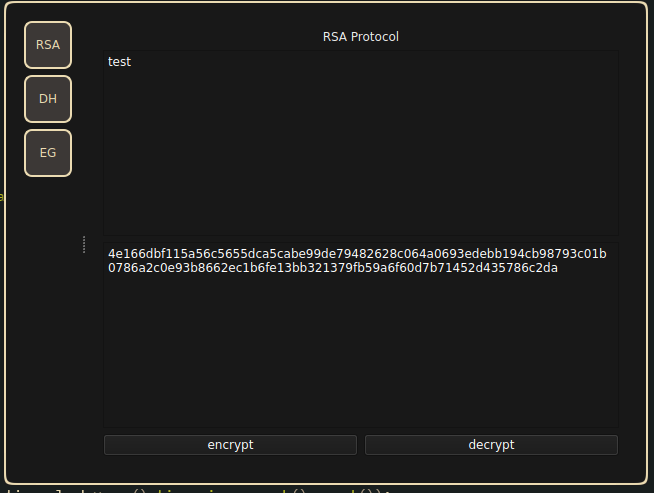
\includegraphics[width=0.48\textwidth]{res/png/00_rsa_encrypt.png}\label{fig:sub1}}
    \hfill
    \subfloat[Decryption]{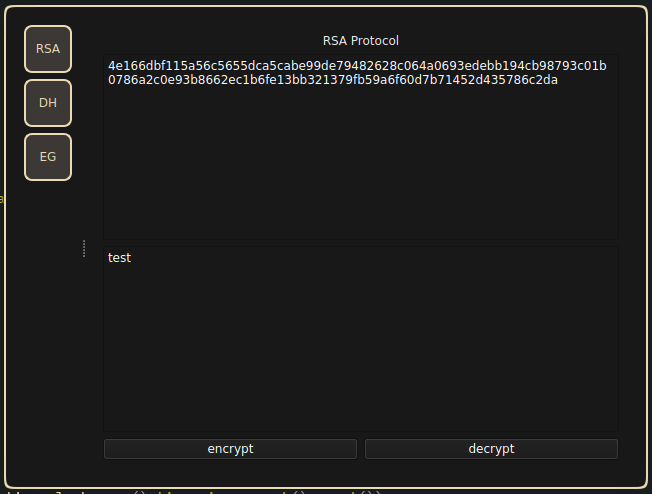
\includegraphics[width=0.48\textwidth]{res/png/01_rsa_decrypt.png}\label{fig:sub2}}
    \label{fig:side_by_side}
\end{figure}
\subsection{Схема шифрования Эль-Гамаля}

Схема шифрования Эль-Гамаля, предложенная Тахиром Эль-Гамалем в 1984 году, является асимметричной криптосистемой, основанной на сложности решения задачи дискретного логарифмирования в конечных полях. В отличие от RSA, это вероятностный алгоритм: одно и то же открытое сообщение может быть зашифровано в множество различных шифртекстов, что повышает его стойкость к криптоанализу.\\

\noindent Рассмотрим реализацию схемы в мультипликативной группе конечного поля $\mathbb{F}_p^*$.

\subsubsection{Генерация публичных параметров}
Перед генерацией ключей для пользователей необходимо создать общий набор параметров, которые будут известны всем участникам системы:
\begin{enumerate}
    \item Выбирается большое простое число $p$.
    \item Выбирается целое число $g$ (называемое генератором или порождающим элементом), которое является порождающим элементом циклической подгруппы порядка $q$ в группе $\mathbb{F}_p^*$.
\end{enumerate}
Параметры $(p, q, g)$ являются открытыми и могут использоваться всеми участниками.

\subsubsection{Алгоритм генерации ключевой пары}
Каждый пользователь (получатель сообщения) генерирует свою пару ключей:
\begin{enumerate}
    \item Выбирается случайное целое число $d$ (секретный ключ), удовлетворяющее условию $1 < d < q$.
    \item Вычисляется открытый ключ $e$ по формуле:
    \[ e \equiv g^d \pmod p. \]
\end{enumerate}
Таким образом:
\begin{itemize}
    \item \textbf{Открытый ключ} — это кортеж $(e, p, q, g)$.
    \item \textbf{Закрытый ключ} — это число $d$.
\end{itemize}

\subsubsection{Алгоритм шифрования}
Для шифрования сообщения $s$ (представленного в виде числа, $1 < s < p$), отправитель использует открытый ключ получателя:
\begin{enumerate}
    \item Выбирается случайное сессионное (эфемерное) число $k$, такое что $1 < k < q$.
    \item Вычисляется первая компонента шифртекста:
    \[ r \equiv g^k \pmod p. \]
    \item Вычисляется вторая компонента шифртекста:
    \[ c \equiv s \cdot e^k \pmod p. \]
\end{enumerate}
Шифртекстом является пара чисел $(r, c)$.

\subsubsection{Алгоритм расшифрования}
Получив шифртекст $(r, c)$, получатель использует свой секретный ключ $d$ для восстановления исходного сообщения $s$:
\[ s \equiv c \cdot r^{-d} \pmod p. \]
Здесь $r^{-d}$ — это мультипликативное обратное к $r^d$ по модулю $p$.\\

\noindent Корректность расшифрования обеспечивается следующими преобразованиями:
\[ c \cdot r^{-d} \equiv (s \cdot e^k) \cdot (g^k)^{-d} \equiv s \cdot (g^d)^k \cdot g^{-kd} \equiv s \cdot g^{dk} \cdot g^{-dk} \equiv s \cdot g^{0} \equiv s \pmod p. \]

\subsubsection{Криптостойкость и особенности}
Безопасность схемы Эль-Гамаля целиком основывается на вычислительной сложности \textbf{задачи дискретного логарифмирования (DLP)}. Зная открытые параметры $(p, q, g)$ и открытый ключ $e$, злоумышленник для нахождения секретного ключа $d$ должен решить уравнение $e \equiv g^d \pmod p$. Для достаточно больших $p$ и $q$ эта задача считается неразрешимой за приемлемое время.\\

\noindent Схема имеет две важные особенности:
\begin{itemize}
    \item \textbf{Вероятностный характер.} Из-за использования случайного числа $k$ при каждом шифровании, одно и то же сообщение $s$ преобразуется в разные шифртексты. Это свойство защищает от атак, основанных на частотном анализе.
    \item \textbf{Удвоение размера.} Шифртекст $(r, c)$ состоит из двух чисел, поэтому его размер вдвое превышает размер исходного сообщения $s$. Это является основным недостатком схемы, ограничивающим её применение для шифрования больших объёмов данных.
\end{itemize}
\subsection{Программная реализация Диффи-Хеллмана}

\subsubsection{Структура класса и зависимости}
Реализация протокола инкапсулирована в класс `DiffieHellman`, который, аналогично `RSA`, наследуется от абстрактного базового класса `Protocol`. Это обеспечивает унифицированный интерфейс для всех криптографических протоколов в системе. Для работы с большими числами, необходимыми для криптографической стойкости, используется библиотека `Boost.Multiprecision` с типом `BigInt`. Интеграция с пользовательским интерфейсом Qt обеспечивается за счет использования типа `QString` для текстовых данных.

\begin{nvimstyle}
#ifndef DIFFIE_HELLMAN_HPP
#define DIFFIE_HELLMAN_HPP

#include "protocol.hpp"

#include <boost/multiprecision/cpp_int.hpp>
#include <boost/random/mersenne_twister.hpp>

using BigInt = boost::multiprecision::cpp_int;

namespace CRYPTO
{
class DiffieHellman final : public Protocol
{
public:
	explicit DiffieHellman(unsigned int prime_bits = 512);
	void init() override;
\end{nvimstyle}

\begin{nvimstyle}
	QString encrypt(const QString& plaintext) override;
	QString decrypt(const QString& ciphertext) override;

	void generateSharedSecret();

	BigInt getPrime();
	BigInt getPublicKey() const;

	void setOtherPartyPublicKey(const BigInt& key);
	void setOtherPartyPrime(const BigInt& prime);

private:
	void generateParameters();
	void generateKeys();
    
	BigInt generatePrime(unsigned int bits, boost::random::mt19937& rng);

private:
	// --- Параметры и ключи Диффи-Хеллмана ---
	unsigned int m_prime_bits;

	// Публичные параметры, общие для обеих сторон
	BigInt m_p; // Простое число-модуль `p`
	BigInt m_g; // Первообразный корень (генератор) `g`

	// Ключи этого участника
	BigInt m_private_key; // Закрытый ключ (секретное число `a` или `b`)
	BigInt m_public_key;  // Открытый ключ (A = g^a mod p или B = g^b mod p)

	// Данные, полученные от другого участника
	BigInt m_other_party_public_key; // Открытый ключ другого участника (A или B)

	// Финальный результат
	BigInt m_shared_secret; // Общий секретный ключ `s = (B^a) mod p = (A^b) mod p`
};

} // namespace CRYPTO

#endif // DIFFIE_HELLMAN_HPP
\end{nvimstyle}

\subsubsection{Инициализация и генерация ключей}
В отличие от RSA, где одна сторона генерирует пару ключей, в протоколе DH каждый участник (назовем их Алиса и Боб) выполняет свой собственный процесс генерации. Этот процесс реализован в методе `init()`, который вызывает внутренний метод `generateParametersAndKeys()`.

\begin{enumerate}
    \item \textbf{Согласование публичных параметров.} На первом этапе обе стороны должны согласовать два числа: большое простое число $p$ (модуль) и целое число $g$ (генератор или первообразный корень по модулю $p$). В данной реализации каждый участник генерирует свое простое число $p$ с помощью вспомогательного метода `generatePrime()`, который использует тест Миллера-Рабина для проверки на простоту. Для симуляции предполагается, что участники "договариваются" об использовании одного из этих наборов параметров (на практике параметры $p$ и $g$ часто стандартизированы и общеизвестны). В качестве генератора $g$ для простоты используется константное значение $5$.

    \item \textbf{Генерация секретного ключа.} Каждый участник генерирует свой собственный секретный ключ — случайное целое число. Алиса генерирует число $a$, а Боб — $b$. Эти числа должны находиться в диапазоне $[2, p-2]$ и храниться в строжайшем секрете.
    
    \item \textbf{Вычисление открытого ключа.} Используя публичные параметры и свой секретный ключ, каждый участник вычисляет свой открытый ключ.
    \begin{itemize}
        \item Алиса вычисляет: $A = g^a \pmod{p}$
        \item Боб вычисляет: $B = g^b \pmod{p}$
    \end{itemize}
    Для выполнения модульного возведения в степень используется оптимизированная функция `boost::multiprecision::powm`.
\end{enumerate}

\begin{nvimstyle}
void DiffieHellman::generateParameters()
{
	boost::random::mt19937 rng(std::random_device {}());

	// Шаг 1: Генерация большого простого числа p
	m_p = generatePrime(m_prime_bits, rng);

	// Шаг 2: Выбор генератора g
	m_g = 5;
}

void DiffieHellman::generateKeys()
{
	boost::random::mt19937 rng(std::random_device {}());

	// Шаг 3: Генерация закрытого ключа `a`
	boost::multiprecision::uniform_int_distribution<BigInt> dist(2, m_p - 2);
	m_private_key = dist(rng);

	// Шаг 4: Вычисление открытого ключа A = g^a mod p
	m_public_key = boost::multiprecision::powm(m_g, m_private_key, m_p);
}
\end{nvimstyle}

\subsubsection{Обмен ключами и вычисление общего секрета}
После генерации ключей участники обмениваются своими открытыми ключами ($A$ и $B$) по публичному каналу. Процесс обмена и последующего вычисления общего секрета управляется классом `DiffieHellmanExchanger`.

\begin{enumerate}
    \item \textbf{Обмен.} Алиса отправляет Бобу свой открытый ключ $A$, а Боб отправляет Алисе свой ключ $B$. В программной реализации это симулируется вызовом метода `setOtherPartyPublicKey()`.

    \item \textbf{Вычисление общего секрета.} Получив открытый ключ другой стороны, каждый участник может вычислить общий секретный ключ $s$. Важнейшим свойством протокола является то, что обе стороны получают одинаковый результат, выполняя вычисления независимо друг от друга.
    \begin{itemize}
        \item Алиса вычисляет: $s = B^a \pmod{p} = (g^b)^a \pmod{p}$
        \item Боб вычисляет: $s = A^b \pmod{p} = (g^a)^b \pmod{p}$
    \end{itemize}
    В результате $s = g^{ab} \pmod{p}$ становится их общим секретом. Злоумышленник, перехвативший $p, g, A, B$, не может легко вычислить $s$, так как для этого ему потребуется решить задачу дискретного логарифмирования (найти $a$ из $A$ или $b$ из $B$).
\end{enumerate}

\begin{nvimstyle}
void DiffieHellman::generateSharedSecret()
{
	if (m_other_party_public_key == 0)
	{
		throw std::runtime_error("Открытый ключ другого участника не установлен.");
	}

	// Вычисление общего секрета: s = (B^a) mod p
	m_shared_secret = boost::multiprecision::powm(m_other_party_public_key, m_private_key, m_p);
}
\end{nvimstyle}


\subsubsection{Использование общего секрета для шифрования}
Протокол Диффи-Хеллмана предназначен исключительно для обмена ключами и не является протоколом шифрования. Однако для демонстрации успешного установления общего секрета были реализованы методы `encrypt()` и `decrypt()`, которые используют полученный ключ $s$ для симметричного шифрования.

\begin{enumerate}
    \item \textbf{Преобразование данных.} Входная строка `QString` преобразуется в массив байтов `QByteArray` в кодировке UTF-8, а затем в большое целое число `BigInt`.
    
    \item \textbf{Операция шифрования/расшифрования.} В качестве симметричного шифра используется простая операция побитового исключающего "ИЛИ" (XOR) между числовым представлением сообщения и общим секретным ключом $s$.
    \begin{itemize}
        \item Шифрование: `ciphertext\_int = plaintext\_int XOR s`
        \item Расшифрование: `plaintext\_int = ciphertext\_int XOR s`
    \end{itemize}
    Так как операция XOR является обратимой, один и тот же метод фактически выполняет и шифрование, и расшифрование.

    \item \textbf{Формат передачи.} Для передачи зашифрованные данные преобразуются в шестнадцатеричную строку. При расшифровании выполняется обратное преобразование из шестнадцатеричной строки в `BigInt`.
\end{enumerate}

\subsection{Пример работы протокола Диффи-Хеллмана}
На рисунке ниже продемонстрирован интерфейс виджета, симулирующего работу протокола. После нажатия на кнопку "Выполнить обмен ключами (DH)" в логе отображается процесс установления общего секрета. Затем Алиса и Боб могут обмениваться зашифрованными сообщениями, подтверждая, что они обладают одним и тем же ключом.

\begin{figure}[htbp]
    \centering 
    \subfloat[Key exchange]{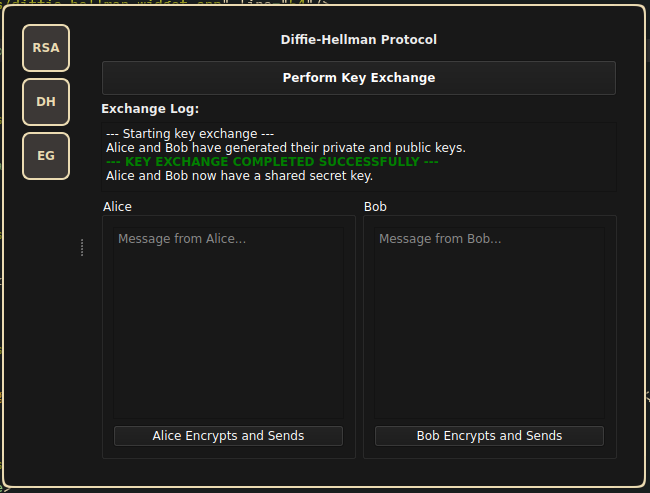
\includegraphics[width=0.48\textwidth]{res/png/04_dh_key_exchange.png}\label{fig:sub1}}
    \hfill
    \subfloat[Message exchange]{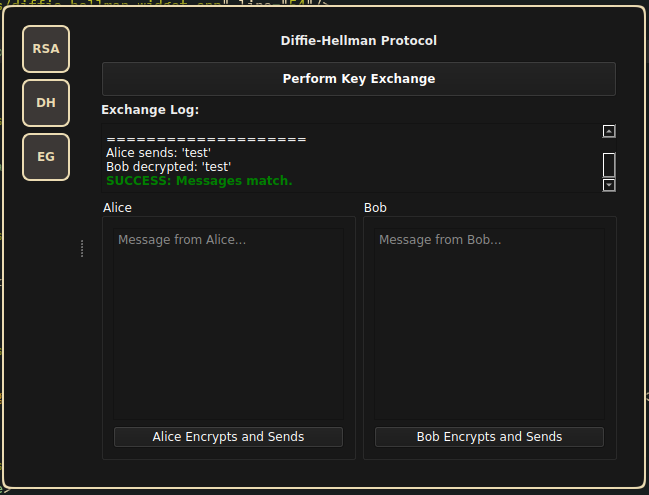
\includegraphics[width=0.48\textwidth]{res/png/05_dh_message_send.png}\label{fig:sub2}}
    \label{fig:side_by_side}
\end{figure}